% Created 2023-02-16 Thu 10:50
% Intended LaTeX compiler: pdflatex
\documentclass[11pt]{article}
\usepackage[utf8]{inputenc}
\usepackage[T1]{fontenc}
\usepackage{graphicx}
\usepackage{grffile}
\usepackage{longtable}
\usepackage{wrapfig}
\usepackage{rotating}
\usepackage[normalem]{ulem}
\usepackage{amsmath}
\usepackage{textcomp}
\usepackage{amssymb}
\usepackage{capt-of}
\usepackage{hyperref}
\author{Filipa  Calado}
\date{\today}
\title{}
\hypersetup{
 pdfauthor={Filipa  Calado},
 pdftitle={},
 pdfkeywords={},
 pdfsubject={},
 pdfcreator={Emacs 26.2 (Org mode 9.1.9)}, 
 pdflang={English}}
\begin{document}

\tableofcontents

\section{"'Where there is Spectacular Passion, they would Suggest Something Vile': Encoding Queer Erasure in Oscar Wilde’s \emph{The Picture of Dorian Gray}"}
\label{sec:orgb48d5d1}

\subsection{Abstract}
\label{sec:orga072e40}
Literary and textual scholars have long speculated about Oscar Wilde's
intentions for revising the homoerotic content of his famous novel,
\emph{The Picture of Dorian Gray} (1891). More recently, electronic editing
standards enable scholars to explore textual composition histories
within a digital space. This chapter explores the Text Encoding
Initiative (TEI) method, an electronic editing tool, for "marking up"
Wilde's revisions to the first chapter of the novel, which introduces
the story's three main characters, Basil Hallward, Lord Henry Wotten,
and Dorian Gray. Drawing from debates in Textual Scholarship and Queer
Studies, I trace what I see as a shared impulse between recovery, that
is, the goal of discovering and preserving origins, and productivity,
or the goal of transforming text for new kinds of analysis. 

Then, I test the TEI's capability in marking up the queer themes in
Wilde's revision. Here, I propose a TEI customization that pushes
against what I identify as TEI's main constraint, which is its
limitation for handling data that is discrete, rather than smooth or
ambiguous data, like the homoeroticism of this text. Like my critique
of text analysis in the previous chapter, this constraint reveals a
connection to queerness: As a labeling tool, the TEI surfaces moments
where queer themes, which are plural and permeable in this text,
threaten to spill over the bounds of its data structure. This
experiment in "queer encoding" shows the limits of the strict data
structure of the TEI for engaging the fluidity and complexity of
queerness in the text.

In my concluding section, I delve into the mutually reinforcing nature
of dominance structures across data formats and text encoding
practices. Here, I draw from critical work on the archive of slavery
to energize a radical re-thinking of editorial practices. I close by
highlighting examples of current projects that deploy collaborative
and minimalist editorial practices to challenge the structuring modes
of textual editing.

\subsection{Introduction}
\label{sec:org8692cd0}
In the first scene of the novel, \emph{The Picture of Dorian Gray} (1891),
the painter Basil Hallward confesses to his friend Lord Henry Wotton
why he cannot exhibit the portrait of the eponymous hero. Basil
admits, "Where there is merely love, they would see something evil,
where there is spectacular passion, they would suggest something vile"
(Wilde 21). This striking line, which provokes the boundary between
aesthetics and romance in a novel that famously luxuriates in paeans
to Hellenic ideals of beauty and hedonism, never appears in print. It
is excised during Oscar Wilde's revision process, along with similar
suggestions of homoeroticism between the three main characters of the
story.

The textual scholarship on this revision process generally agrees that
Wilde neutralizes Basil's erotic fascination with Dorian by
transforming it into aesthetic appreciationas as part of a larger
purpose to get by the censors. Further transformations suppressed
homosexual themes in the text into a cypher. Like in the text's
"Preface," which was included with the book version published in 1891:
"To reveal art and conceal the artist is art's aim," and "Those who
find ugly meanings in beautiful things are corrupt without being
charming." One critic, Nicolas Ruddick, explains that Wilde's revision
process for this text instantiated a double moral, one about beauty
and one about sexuality. According to Ruddick, Wilde revisions
increasingly aestheticize Dorian in order to emphasize a moral about
the dangers of vanity at the expense of another, more covert moral
about the liberalization of homosexuality. While the moral about
vanity "dramatize[s] the disastrous consequences of the preference of
the beautiful at the expense of the good," the other moral about
homosexuality "explores the destructive effects of the clandestine or
closeted life" (Ruddick 126, 128). The novel's famous portrait indexes
the convergence of these two morals: "the appalling changes to
Dorian's painted image \ldots{} strongly suggest that the unspeakable
practices indulged in by the protagonist are unspeakable in
themselves" (Ruddick 129).

The question of what is "unspeakable," and why, about the homosexual
suggestsions in Oscar Wilde's text is the topic of this chapter. To
explore these revisions, I use a digital editing technology to mark
and categorize them according to themes like "passion," "beauty,"
"intimacy," and "fatality." But what begun as a textual editing
project eventually expanded into an interrogation of the electronic
editing tool that I used to digitize the text, the Text Encoding
Initiative (TEI). I found that the rigid, hierarchical structure of
the TEI's data format works best with material that is discrete, and
can be separated into distinct elements, rather than smooth data, like
the queer themes of the text. As a labeling tool, I found that the TEI
indexes moments of plurality and permeability, when themes like
"intimacy" and "fatality" threaten the bounds of the strictly
delineated data structure. 

Then, as I delved deeper into the data structure of the TEI, I found
the problem goes deeper than bounding or containing textual
data. Because hierarchical structures are totalizing, they impose a
dynamic of dominance and submission between all elements within the
system. Therefore, I propose that underlying Ruddick's two morals
about beauty and homosexuality, there is a third level of
"unspeakability," this one about power, about who has it and who is
subject to it.

\subsubsection{Is markup 'queerable'?}
\label{sec:org08de0c6}
My project endeavors to answer a question posed by literary and
electronic textual scholar Julia Flanders: "do we need to queer
markup, or is markup already queerable?" (2017). Flanders's question
considers the TEI's place between two current approaches in Queer DH:
the first approach wants to disrupt formal systems by imagining
alternative ones, and the second, by contrast, maintains that
queerness is built into computing and is inherent in computational
logic.\footnote{See introduction for a more detailed explanation of this
tension.} In an attempt to cut between these debates, this project
first searches for a structural constraint within the TEI format, and
then works through this constraint to analyze the homoerotic elements
in Wilde's manuscript revisions. As such, this project aligns Jason
A. Boyd's \emph{Texting Wilde Project}, uses the TEI to destabilize current
understanding of Wilde's textual and historical legacy. Boyd's
project, which marks up the biographical information, particularly
references to persons, places, and events, in writings about Wilde's
life, reveals the historical discrepencies and inaccuracies across
Wilde's biography. Boyd points out that "Our knowledge of 'Oscar
Wilde' is not comprised of a corpus of pure and simple facts that
allows us an unmediated apprehension of a real person separated from
us by only time, but rather this knowledge is comprised of a densely
complex and often contradictory accretion of texts" (Boyd para. 1).

Similar to Boyd, my project also uses the TEI to complicate the
understanding of Wilde's textual legacy. It identifies one major
constraint of the TEI: that it works best with data that is discrete,
rather than smooth data, like the homoeroticism obscured by Wilde's
pen. Here, I apply the rigid constraint of the TEI data structure
towards marking up and analyzing this text's homoeroticism, which I
group into the general themes of "intimacy," "beauty," "passion," and
"fatality," as well as the pen strokes that Wilde used to strike these
elements from the text. The functionality of the TEI as a tool that
bounds and labels data into discrete elements allows me to explore the
indeterminate boundaries of these queer themes in the text. The strict
nature of this tool also suggests, on a deeper level, how dominance
structures work to implicitly determine and delimit information. 

\subsection{Textual Scholarship and Queer Historiography}
\label{sec:orgbc8bde5}
To inform my approach for handling homoerotic subject matter within
digital contexts, I bring Textual Scholarship and Queer Historiography
into conversation. Between these two fields, I identify a parallel
debate between what I term the "restorative" and "productive"
approaches to critical analysis.

The history of Textual Scholarship first tends toward the restorative
approach, beginning with the work of Shakepearean scholar Ronald
B. McKerrow, who maintains that the goal of scholarly editing is to
preserve authorial intention. McKerrow's influential model for
"copy-text" editing, which establishes the base-text for editing on an
early witness that most closely resembles the author's original
intention, eventually gives way to Walter W. Greg's approach that
expands the purview of critics to more than a single
witness. Subsequently, textual scholars like Fredson Bowers and Thomas
Tanselle advance Greg's work, proposing the "eclectic edition" as the
format that enables the editor to distil authorial intention from
multiple sources.\footnote{See McKerrow, Bowers, and Tanselle.} Tanselle in particular takes this principle to
its logical conclusion, arguing that the "work" exists in an ideal
form, beyond the reach of physical corruption:
physical corruption: 
\begin{quote}
Those who believe that they can analyze a literary work without
questioning the constitution of a particular written or oral text of it
are behaving as if the work were directly accessible on paper or in
sound waves \ldots{} its medium is neither visual nor auditory. The medium of
literature is the words (whether already existent or newly created) of a
language; and arrangements of words according to the syntax of some
language (along with such aids to their interpretation as pauses or
punctuation) can exist in the mind, whether or not they are reported by
voice or in writing. (Tanselle, 1989: 16--17)
\end{quote}
Tanselle's position enshrines the editor as the only figure capable of
realizing the "work" in its ideal form. Because the act of inscription
involves physical tools that can corrupt this ideal form, the writer
requires an editor whose distance from the creation of the work
enables his objective evaluation of its intention. Tanselle's quite
radical view for preserving authorial intention exemplifies the
extreme of the restorative approach.

If the restorative approach promotes editorial practices that
increasingly consign the role of the editor as a recoverer or
preserver of texts, the productive approach empowers the editor as an
enabler of potential textual readings. Toward the end of the 20th
century, textual scholar D. F. McKenzie's ideas about "the sociology
of texts" were the first to widely challenge the claim that a single
text can represent an "ideal" version, that is, authorial
intention. According to McKenzie, the text is never one single object
but stems from a number of human agencies and mechanical techniques
that are historically situated; he points out that, "Every society
rewrites its past, every reader rewrites its texts, and if they have
any continuing life at all, at some point every printer redesigns
them" (McKenzie 25). Jerome McGann expands this sociological
perspective into digital editing environments, where electronic
formats create opportunities for presenting textual variation. McGann
explains that textual criticism in print format is limited because a
print text must conform to the linear and two-dimensional form of the
codex--the same form as its object of study. Digital editions, by
contrast, can be designed for complex, reflexive, and ongoing
interactions between reader and text. McGann notes that his work on
the digital \emph{Rossetti Archive} brought him to repeatedly reconsider
his earlier conception and goals, explaining that the archive "seemed
more and more an instrument for imagining what we didn't know" (McGann
82). McGann's approach counters the traditional fidelity toward
authorial intention with a drive to harness the potentiality of
textual variation. The transformation of literary material into
electronic format becomes a vehicle for a critical analytical method
that McGann and Lisa Samuels call "deformative criticism," which works
by distorting, disordering, or re-assembling literary material in
order to estrange the reader from their familiarity of the
text. Continually subscribing the text to new configurations, this
estrangement confronts the reader with new insights about its formal
significance and meaning.

My work encoding Wilde's revisions to the manuscript plays against the
long-standing "recovery" project about Wilde's intentions as he
revises \emph{Dorian Gray} into the periodical and book versions. Textual
scholars like Donald Lawler, Joseph Bristow and Nicolas Ruddick claim
that Wilde's revisions work toward the overall goal of aestheticizing
the text. This project of aestheticization begins in the manuscript
which is eventually published, in periodical form, in \emph{Lippincott's
Monthly Magazine} on June 20, 1890.\footnote{See Frankel, pp. 40–54, for a more complete accounting of the
role of John Marshall Stoddart (Wilde’s publisher) in preparing the
typescript for publication.} This first printing of ‘The
Picture of Dorian Gray', which spans 98 pages over 13 chapters, was
widely criticized in the press for its seemingly ambiguous stance on
an immoral protagonist. Bristow explains that ‘[Wilde's] narrative
struck the [reviewers] as a work that appeared “corrupt”, displayed
“effeminate frivolity”, and dealt “with matters only fitted for the
Criminal Investigation Department”' (2000: xviii). Wilde spends the
next several days defending his work in letters to the editors,
entering into a public correspondence with them.\footnote{See Wilde, O and M P Gillespie, pp. 358--374, for a selected list of
full-length reviews from \emph{The Scots Observer, The St James Gazette} and
the \emph{Daily Chronicle}, and Wilde's responses.} A few months
later, in the early spring of 1891, Wilde publishes a ‘Preface' that
makes such claims as ‘Those who find ugly meanings in beautiful things
are corrupt without being charming. This is a fault' and ‘To reveal
art and conceal the artist is art's aim'.\footnote{See Wilde, O and M P Gillespie, pp. 3--4.} Scholar Barbara
Lecklie asserts that, by these complex and incisive statements,
‘Wilde's strategy is to refocus on art and disparage the focus on the
reader by saying that the reader is the one who makes a work immoral'
(2013: 173). Similarly, Lawler argues that ‘the “Preface” \ldots{} hold[s]
up aesthetic beauty and artistic effect as the only legitimate
criteria of critical evaluation' (1988: 16). The ‘Preface' is included
in the subsequent iteration of \emph{Dorian Gray}, published in a book
version by Ward, Lock \& Company in April 1891. According to the editor
of the \emph{Uncensored Edition} of \emph{Dorian Gray}, Victor Frankel, Wilde
here makes significant deletions of passages referencing
homosexuality, promiscuous or illicit heterosexuality, and ‘anything
that smacked generally of decadence' (2011: 47--48). Wilde also
‘heighten[s] Dorian's monstrosity toward the novel's conclusion' to
bring the story ‘to a moral conclusion that he thought would silence
his critics' (Frankel, 2011:30).

Like Textual Scholarship, the field of Queer Historiography has also
engaged in debates about methodologies for recovery. Susan McCabe
describes "Queer Historiography" as the "critical trend of locating
'identifications' (rather than identity), modes of being and having,
in historical contexts." Within this field, there is a debate about
the extent to which critics in the present can adequately define
queerness in the past (McCabe 120). The Queer Historicist position
advocated by scholars like David Halperin and Valerie Traub maintain
that homosexuality is historically constructed, that "queerness" means
something different today than it did in the past, and that scholars
can get at its meaning by employing a Foucauldian genealogical method
that traces its meaning over time. Identity based on sexuality,
according to Halperin, is a modern cultural production: "no single
category of discourse or experience existed in the premodern and
non-Western worlds that comprehended exactly the same range of
same-sex sexual behaviors \ldots{} that now fall within the capacious
definitional boundaries of homosexuality" (Halperin 88). Evoking
Judith Butler's famous description on the word "queer" as "never fully
owned, but always and only redeployed, twisted, queered from a prior
usage and in the direction of urgent and expanding political
purposes," Valerie Traub explains that the utility of the word "queer"
as a descriptive term relies on historical specificity (173):
\begin{quote}
Queer's free-floating, endlessly mobile, and infinitely subversive
capacities may be strengths---allowing queer to accomplish strategic
maneuvers that no other concept does---but its principled imprecision
implies analytic limitations \ldots{} if queer is intelligible only in
relation to its social norms, and if the concept of normality itself
is of relatively recent vintage (Locherie), then the relations between
queer and the changing configurations of gender and sexuality need to
be defined and redefined. Traub 33
\end{quote}
When "queer" is applied ahistorically, it loses its descriptive
value. According to this historicist position, homosexuality, in order
to be legible, necessitates historical specificity.

By contrast, the "unhistoricists" are wary of demarcating queer
identity and identification across history. These scholars, who
include Jonathan Goldberg, Madhavi Menon, and Heather Love, maintain
that the attempt to define "queer" implicitly subscribes queerness to
a logic of progress, a heteronormative teleology. Historicizing
queerness has the effect of normalizing queerness, according to
Goldberg and Menon: "to produce queerness as an object of our scrutiny
would mean the end of queering itself" (1609, 1608). Within this view,
Heather Love offers an opportunity for continuing the project of queer
history. Her methodology takes negative affects like shame, anger,
disgust, hatred, disappointment as part of an accounting of "the
social, psychic, and corporeal effects of homophobia" (2). This
method, which she calls "feeling backward," takes negative affects and
histories without attempting to "fix" them into contemporary
conceptions of identity and desire. Rather, Love is interested in
exploring the way that subjects turn away or refuse the critic's
attempt to "redeem" or "rescue" them. To illustrate this process of
"feeling backward," she offers the myth of Orpheus and Eurydice,
pointing out that Orpheus \emph{prefers} to behold Eurydice in the darkness
of the Underworld rather than in the sunlight, which would transform
her into something fully accessible and therefore less
desirable.\footnote{As the condition of rescuing his lover Eurydice from Hades, Orpheus
must not look at her until they exit the Underworld and re-emerge into
the sunlight. Unable to restrain himself, Orpheus turns to gaze at
Eurydice as they are about to pass through the threshold. In this
glimpse he manages to catch of his lover, she is already shrinking away
into the darkness where she will be forever imprisoned.} Love, who asserts that "Queer history has been an
education in absence" (52), points out that "[Eurydice's] specific
attraction for queer subjects is an effect\ldots{} of a historical
experience of love as bound up with loss. To recognize Eurydice as
desirable in her turn away is a way of identifying through that loss"
(51). 

Across Textual Scholarship and Queer Historiography, there are two
parallel methodologies for addressing the problem of what to do with
the past. On the restorative side, the impulse to recover authorial
intention resembles the drive to historicize queer
identification. Both are motivated by a notion that the past is
accessible to the discerning critic. On the productive side,
deformative criticism plays on the same creative instinct as "feeling
backward." Love describes this work as "a mode of historiography that
recognizes the inevitability of a 'play of recognitions' but that also
sees these recognitions not as consoling but as shattering" (Love,
2009: 45). In this "play of recognitions," which describes the
critic's "search for roots and resemblances" within queer subject
matter, I want to emphasize the word "play" (45). The impossibility of
recovering the past enables the critic to experiment with alternative
methods of analysis. For Love, accepting queerness as something that
eludes containment compels her to explore how queerness escapes
knowability. I propose that this method of attending to elusive
affects, without trying to transform them into something more
palatable, can apply to digital contexts and toward productive
ends. One may, borrowing from McGann and Samuel's idea of deformance,
reconceive textual editing as a formal experiment. The TEI can be used
to explore how electronic editing tools impose new formal structures
on queer subject matter. This allows one to take the attempt at
recovery and, rather than aim for resolution, multiply the potential
readings of textual elements. Using the TEI in this way allows
researchers to direct ‘queer encoding' practices toward enacting what
Kadji Amin, Amber Jamilla Musser, and Roy Pérez describe as ‘queer
form', or ‘the range of formal, aesthetic, and sensuous strategies
that make difference a little less knowable, visible, and digestible'
(2017: 235).

An examination of queer form in this text will reveal the ways in
which power is more deeply entrenched than I had anticipated. To
better understand the workings of power in data structures, it is
useful to examine the historiographical work on arguably one of the
most precarious datasets in history—-the archive of slavery. Like
Heather Love, scholar Saidiya Hartman seeks to recuperate (without
recovering) the lives of these subjects. But unlike Love, Hartman's
subjects are constituted in history by their absence in the
archive. Hartman's question haunts all historiographical work in this
area: "How does one revisit the scene of subjection without
replicating the grammar of violence?” (4). She explains that the
"violence of the archive" is a double erasure---not only does the
archive omit or obscure information, but it also employs a language
that cannot approximate experience (Hartman 2). Pushing against the
tradition of recording the subject in the terms of their
objectification, in "a display of the violated body, an inventory of
property," Hartman's goal is to write about these subjects in a way
that also invites possibility for living. For doing so, she proposes a
method of "critical fabulation" (2, 11). Like "deformance" and
"feeling backward," her method of "critical fabulation" plays on
imagination and experimentation. But due to the death and violence
that constitutes this archive, formal experimentation is not enough.

\subsection{TEI}
\label{sec:org7b25dde}
Created specifically for working with literary material, the TEI
enables researchers to describe, transcribe and edit print text or
manuscripts in electronic format. The TEI enables users to "mark up"
aspects of literary texts that they think are important, such as
structural elements (chapters, paragraphs, line breaks), physical
details about the text (revisions, illegible text) or conceptual
elements (persons, geographical locations). To mark up these elements,
encoders use "tags." such as \texttt{<line>} to indicate a line of text,
\texttt{<del>} to indicate deleted text, and \texttt{<person>} for a reference to a
person. To illustrate what markup looks like, pictured below is an
image of Mary Shelley's manuscript of \emph{Frankenstein; or, The Modern
Prometheus} (1818) and its diplomatic transcription (see Figure
1). Beneath them is an excerpt of the underlying TEI code, created by
the researchers at the Shelley-Godwin Archive.

Image of the manuscript and diplomatic transcription of \emph{Frankenstein}
(Bodleian MS Abinger c.56: 1816), transcribed and encoded by the
Shelley-Godwin Archive.

\begin{center}
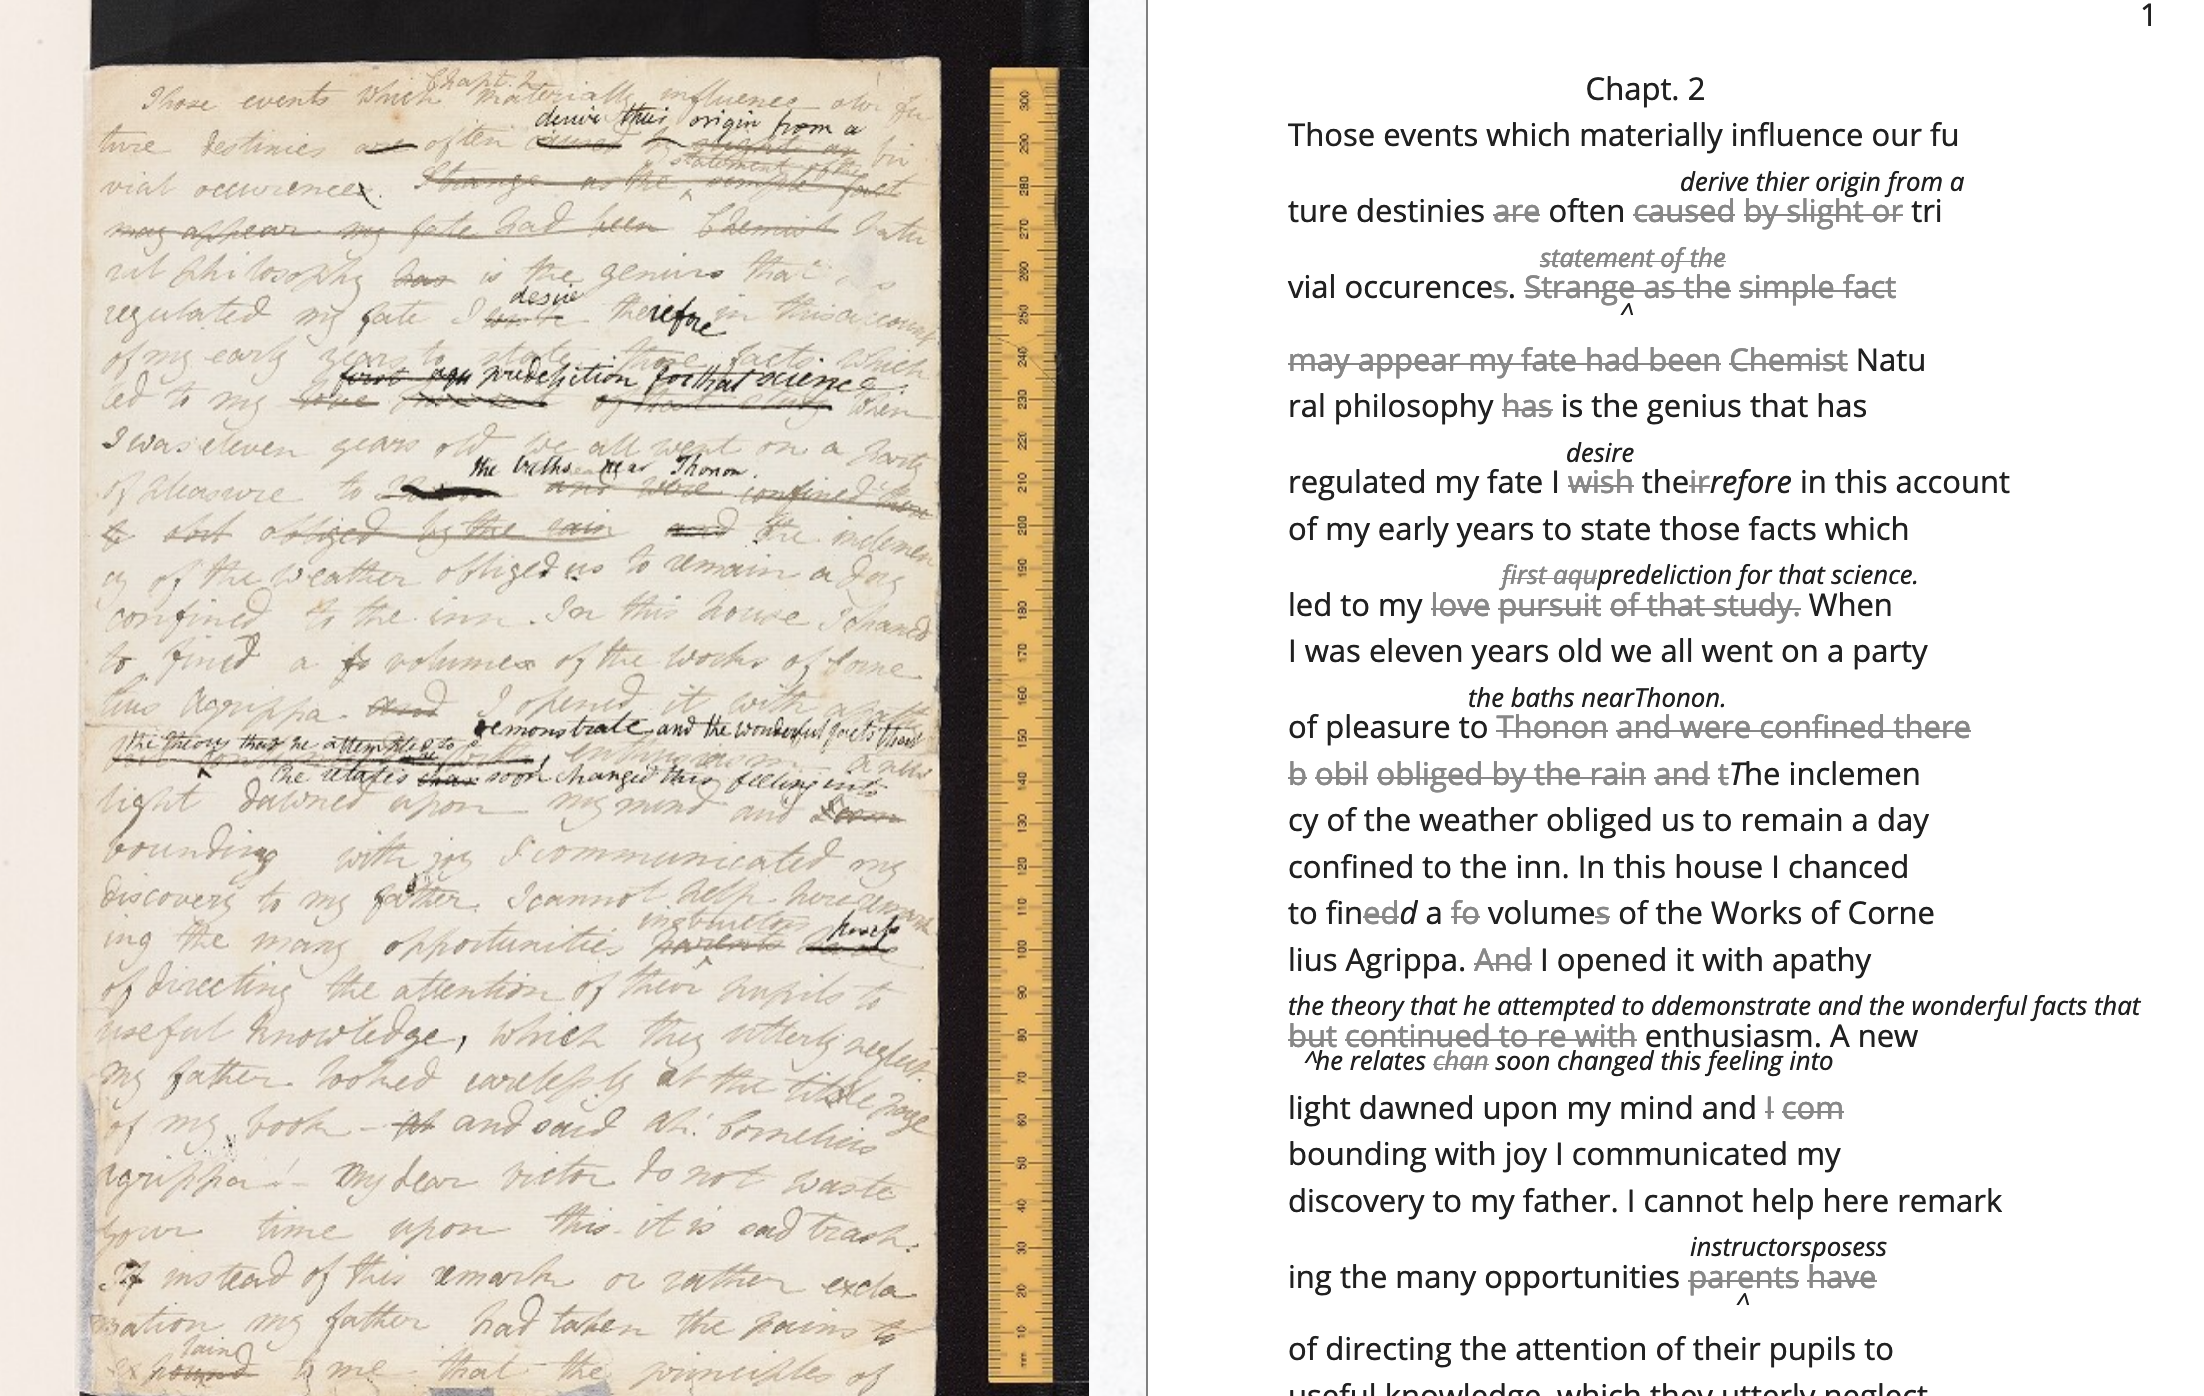
\includegraphics[width=.9\linewidth]{./figure1.png}
\end{center}

\begin{SOURCE}
<handShift medium="pen" new="\#mws"/>

<line>Those events which materially influence our fu</line>

<line>ture destinies <del rend="strikethrough">are</del> often
<mod> <del rend="strikethrough">caused</del>

<del rend="strikethrough">by slight or</del>

<add hand="\#pbs" place=”superlinear”>derive thier origin from a</add>
</mod> tri </line>

<line>vial occurence <del rend="strikethrough">s</del>.

<mod spanTo="\#c56-0005.01"/> <del rend="strikethrough"
next="\#c56-0005.02">Strange as the</del>
\end{SOURCE}

In the encoding, the \texttt{<line>} tags indicate lines of text, and \texttt{<del>}
tags indicate deleted text. Through this level of detail, TEI
facilitates deep and complex description of textual material for
scholarly research. This excerpt also includes a \texttt{<handShift>} tag and
\texttt{@hand} attribute, which indicate whose "hand" is responsible for
writing each section of text: a valuable piece of information for a
text co-edited by Shelley's husband, Percy Shelley.

TEI documents consist of an ordered hierarchy. The document
organization resembles a tree structure, with one "root" component and
several "branches."  The TEI requires that all data be contained as
discrete components within this bounded structure, and they cannot
overlap unless the inner element is fully nested within an outer
element. For example, a \texttt{<del>} element must be fully contained within
its parent element, say a \texttt{<line>} or \texttt{<paragraph>} element, depending
on the document schema.

Implied by this data model is a structure of dominance, where the
higher or "parent" element exerts some control over the lower or
"child" element. Within a hierarchical data model, conflicts arise
when elements overlap, from the clash between structural and semantic
dimensions of the elements. Element overlap is essential for some
forms of written language where textual structure, such as syntax or
grammar, might overlap with semantics. XML researcher Jeni Tennison
points out that, "the way in which the syntactic (sentence/phrase)
structure overlaps with the prosodic (stan/za/line) structure is one
important way in which you can analyse a poem ("Overlap, Containment,
and Dominance"). Tennison, who "want[s] to see if we can get away with
not having hierarchy as a fundamental part of the information model,"
distinguishes dominance from containment:
\begin{quote}
When you’re talking about overlapping structures, it's useful to make
the distinction between structures that \emph{contain} each other and
structures that \emph{dominate} each other. Containment is a happenstance
relationship between ranges while dominance is one that has a
meaningful semantic. A page may happen to contain a stanza, but a poem
domainates the stanzas that it contains. Tennison 2008, "Overlap,
Containment, and Dominance"; emphasis original
\end{quote}
As a solution that prioritizes containment while also suggesting
dominance relationships, Tennison proposes a new (but now unsupported)
markup language: "The Layered Markup and Annotation Language"
(LMNL). It uses a series of ranges that describe start and stop points
for an element, rather than nesting elements one inside the other. In
the example below, the tags are left open to accommodate additional
ranges:
\begin{SOURCE}
[book [title [lang\}en\{lang]\}Genesis\{title]\}
[chapter\}
[section [title\}The creation of the world.\{title]\}
[para\}
[v\}[s\}[note\}In the beginning of creation, when God made heaven and
earth,\{note [alt\}In the beginning God created heaven and
earth.\{alt]]\{v] [v\}the earth was without form and void, with darkness
over the face of the abyss, [note\}and a mighty wind that swept\{note [alt\}and
the spirit of God hovering\{alt]] over the surface of the waters.\{s]\{v]
[v\}[s\}God said, [quote\}[s\}Let there be a light\{s]\{quote], and there
was light;\{v] [v\}and God saw that the light was good, and he separated
the light from darkness.\{s]\{v] [v\}[s\}He called the light day, and the
darkness night. So evening came, and morning came, the first
day.\{s]\{v]
\{para]
\ldots{}\{chapter]\ldots{}\{section]\ldots{}\{book] "The Layered Markup and Annotation
Language (LMNL)" 
\end{SOURCE}
This language indicates dominance relationships through layering
markers, rather than through a tree structure. Despite this feature,
the document object model is considerably less readable than the TEI.

The problem with TEI, and more deeply, with its parent structure, XML,
is that dominance structures are totalizing. Attempts to curtail this
dominance, as LMNL demonstrates, can result in redundancy and
convolution. The TEI Guideline’s suggestions for handling dominance
appear similarly complicated, especially in comparison to more
traditional TEI markup. Module 16, on "Linking, Segmentation, and
Alignment," describes various methods for encoding information that is
not hierarchic or linear, including the use of pointers, blocks,
segments, anchors, correspondence, alignment, synchronization,
aggregation, alternation, sequestration, marginalization, among
others. In Module 20, “Non-hierarchical Structures,” more suggestions
include: “redundant encoding of information in multiple forms," and
"the use of empty elements to delimit the boundaries of a non-nesting
structure.” These solutions work by severing elements into components
that maintain their own internal hierarchies which can be later
recombined into the dominant hierarchy. When the totalizing nature of
the TEI is diluted, the effect is to create a bureaucratization that
disrupts its sense of unity.

Though the strict tagging structure of the TEI forces encoders to
organize textual elements as discrete, ordered data, it also enables
them to create their own labels for the elements. Perhaps the most
useful aspect about the TEI is this customizability, which it inherits
from its parent language, eXtensible Markup Language (XML). As an
"extensible" language, TEI users can create their own tags to describe
the particular elements they wish to encode. \emph{The Women Writers
Project (WWP)}, directed by Julia Flanders, adequately frames how
TEI's inherent extensibility can address textual ambiguity. According
to the \emph{WWP}:
\begin{quote}
Unlike many standardization efforts, the TEI \ldots{} explicitly
accommodat[es] variation and debate within its technical
framework. The TEI Guidelines are designed to be both modular and
customizable, so that specific projects can choose the relevant
portions of the TEI and ignore the rest, and can also if necessary
create extensions of the TEI language to describe facets of the text
which the TEI does not yet address. (Flanders, 1999--2021)
\end{quote}
Because TEI is built from a language that allows its users to build
their own version of that language, there is potential for
representing the elements necessary for a project by customizing these
elements on a project-by-project basis.

There are a number of projects that explore the potential of the TEI's
customization to be used for "queer encoding," such as the encoding of
queer gender. Marion Thain encodes the diaries of a complex writing
subject: the late 19th-century English poet, Michael Field. Michael
Field is a pen name for the lesbian couple, Katharine Bradley and
Edith Cooper, which signifies "the assumed names of two separate
women, as well as appearing to signify one single male identity"
(Thain 228). Fortunately for Thain, the TEI enables the encoding of
distinct identities, which is central for understanding the queerness
of the diaries:
\begin{quote}
[T]he proliferation and slipperiness of names is no mere childish
caprice but a core part of the articulation of queer: an unhinging of
"given" or apparently predetermined identity through a strategy that
articulates identity as constantly shifting, constructed, and
performative. Text encoding can, in a simple but powerful way, help us
explore and map this crucial strand of queer identity construction
across the diary. (Thain 233)
\end{quote}
Thain's approach harnesses the hierarchical nature of the TEI to list
the various references to each personage within the \texttt{<persName>} tag.
This \texttt{<persName>} tag allows Thain to "render searchable words not in
the text but intimately tied to it. This is not a small issue in a
diary in which Katharine Bradley herself is referred to by more than
20 different names" (Thain 233). By enabling Thain to encode multiple
names for each writer of the text, the TEI data structure enables
Thain to manage the problem of queer identity in this text.

While some gender identities may take manifold forms, some of which
can be contained within a capacious enough set of tags and attributes,
other gender identities may not fit into distinct categories. As
gender and queer studies scholars may know, some elements of identity
will resist containment within unified or discrete idea of
subjectivity. In this case, the problem goes deeper than the name of
the tag itself and runs up against the hierarchical structure of the
TEI document model. At the most recent annual TEI Conference and
Members Meeting in 2022, Elisa Beshero-Bondar and her team reflect on
their work developing a \texttt{<gender>} element for the TEI
guidelines. Their project proposes a new \texttt{<gender>} element that is
careful to weigh the expressive potential for representing gender
against the possible risks of reifying normative cultural
biases. Beshero-Bondar and her colleagues explain that,
\begin{quote}
Unexpectedly, we found ourselves confronting the Guidelines’
prioritization of personhood in discussion of sex, likely stemming
from the conflation of sex and gender in the current version of the
Guidelines. In revising the technical specifications describing sex,
we introduced the term “organism” to broaden the application of sex
encoding. We leave it to our community to investigate the fluid
concepts of gender and sex in their textual manifestations of
personhood and biological life. Beshero-Bondar et al.
\end{quote}
While their new proposed element, \texttt{<gender>}, gives the team some
capacity to represent gender as distinct from sex, the tagging
structure nonetheless perpetuates a rule that "sex" serves some
concept of personhood. The proposed solutions to this problem, which
include exchanging \texttt{<person>} for the more capacious \texttt{<organism>} and
\texttt{<entity>}, as recently proposed in the TEI documentation itself,
keeps intact the notion that "sex" is something a person contains,
that is, sex as something belonging to or expressed by a notion of
personhood (martindholmes 2022).

It is safe to say that the TEI works effectively depending on the kind
of queerness that we want to encode. If that queerness resists an idea
of unified or contained personhood, then encoding will be
difficult. For example, tags such as \texttt{<gender>} or \texttt{\textasciitilde{}<person>} limit
elements to one value and creates obstacles for scholars working to
encode multiple or diverse sexual identities. Here, Pamela Caughie and
Sabine Meyer use the the TEI to encode \emph{Man Into Woman}, the life
narrative of Danish painter Lili Elbe, who undertook one of the first
gender affirming surgeries in 1930. The attempt to mark up Elbe's
complex gender ontology brings Caughie and Meyer against this
structural limitation of the TEI:
\begin{quote}
[T]he deeper we got into mark-up, the more evident it became that the
categories and hierarchies available to us were inadequate for our
task\ldots{} to identify a male subject who at times presents himself as
masquerading as a woman, at others as being inhabited by one, and who
eventually becomes a woman, in a life history narrated retrospectively
from the perspective of Lili Elbe. (Caughie and Meyer, 2018: 231)
\end{quote}
The limitations of the \texttt{<gender>} tag forces these scholars to
consider the ways that the TEI effectively reifies gender as
essential. For this project, the fixity that the TEI imposes upon Elbe
as a queer subject brings out the ways that gender is situated and
relational across this text. 

Why do Caughie and Meyer struggle to encode Elbe's identity while
Thain appears to succeed with Fields'? This question about the TEI's
capacity to adequately categorize queer identity points to a deeper
problem within hierarchical data structures. While a queerness like
Fields' might be delineated and contained, in Elbe's there is a
quality of blending which the markup, by its nature, means to separate
and fix. Fields' identity is multiple yet distinct: the diaries
proffer "two different hands [that] record the experience of two
clearly differentiated people" (Thain 229). By contrast, Elbe's
identity is plural, containing several identities whose relationship
to each other is ambiguous or continually shifting within one
entity. Elbe's relation to gender is best described qualitatively, as
one that alternatively "masquerades" or "inhabits" simultaneous gender
ontologies (Caughie and Meyer 231). Because of the TEI's dominance
dynamic, in which one element must take precedence over a subordinate
one, elements must be totally bounded and contained within the overall
structure.

\subsection{The Manuscript of \emph{Dorian Gray}}
\label{sec:org3124c74}
For Wilde's text, I created a TEI customization that explores the
potential of semantic labeling against the demands for fixity and
structure within the TEI data structure. My customization registers
physical and conceptual changes to the manuscript by creating two new
attributes to mark the revisions. First, the custom attribute
\texttt{@implication} marks the general theme of revision from a list of
recurring themes, which include: "intimacy," "beauty," "passion," and
"fatality," with the additional values of "inconclusive," "unclear" or
"illegible." Then, to mark the physical traces of Wilde's pen as he
struck out portions of the text, I created the custom attribute
\texttt{@strokes} that registers the number of pen strokes through any given
section of text.\footnote{I am grateful to Jason A. Boyd for making this suggestion.} Most often, Wilde uses one or two strokes of
his pen, although sometimes, the strokes are too heavy or thick to
enumerate. In those cases, I set the \texttt{@strokes} attribute to the value
"inconclusive." Below is an example of how the markup applies to a
section of Wilde's manuscript. Here, I use default elements and
attributes to mark the revisions, such as \texttt{<mod>}, \texttt{<add>}, \texttt{<del>},
as well as the built-in \texttt{@rend}, and \texttt{@place} attributes, to which I
add my custom attributes, \texttt{@implication} and \texttt{@strokes}.

\begin{SOURCE}
<quote> The ugly and the stupid have the best of it in this
world. They can sit quietly, and gape at the play. If they know
nothing of victory, they are 

<mod type="subst"> 

<del rend="strikethrough"> <unclear>saved</unclear> </del> 

<add>at least spared</add> </mod> 

the knowledge of defeat. They live as we all should live, undisturbed,
indifferent, and without disquiet. They neither bring ruin upon
others, nor ever receive it from alien hands. Your rank and wealth,
Harry; my brains, such as they are, my fame, whatever it may be worth;
Dorian Grey's 

<mod type="subst"> <del rend="strikethrough" strokes="2"
implication="beauty">beauty;</del> 

<add place="above">good looks;</add> </mod> 

we will all suffer for what the Gods have given us, suffer terribly."
</quote>
\end{SOURCE}

In what follows, I detail how this customization registers the
elisions of homoeroticism in the manuscript as Wilde prepared it for
publication. Here, the difficulty is in engaging the boundedness of
the TEI elements, which encapsulate data, with the indistinctiveness
of the queerness of the text, which resist demarcation. The four
themes of "intimacy," "beauty," "passion," and "fatality" constitute a
spectrum of smooth information that threatens the confines of the TEI
tags. To add another layer of ambiguity, the number of pen strokes
also resists easy demarcation: they can be difficult to enumerate and
their boundaries often fail to map with the themes. The goal of this
work is not to establish a formal method for marking queer elements,
rather, it is to surface a resistance in the text: an indeterminacy
that resists capture by the TEI data structure.

The evocative opening scene, which consists of a lively dialogue
between Basil Hallward and Lord Henry Wotton, sets the tone, reveals
character dynamics, and lays out some of the conflict for the ensuing
story. In these first few pages, Basil appears to be a sympathetic,
sensitive, albeit slightly exasperated artist, who confides in his
close friend Lord Henry the powerful influence that Dorian Gray has
had upon his life and work. Lord Henry, by contrast, appears as an
affable and witty gentleman aesthete, who counters Basil's sincerity
with offbeat observations and paradoxical aphorisms. From the
revisions that Wilde made to this opening scene, a few general
patterns emerge. First, the revisions work to stifle the emotional
tension and physical affection in the dialogue between Basil and Lord
Henry, replacing it with a lighter or more neutral tone. Because such
revisions generally shore up the friendship between Basil and Lord
Henry, conveying fondness in their rapport, they are encoded according
to the theme of "intimacy." Second are the themes of "beauty" and
"passion," which mostly concern revisions where Dorian is reformulated
from a romantic object into an artistic subject for Basil's
painting. Third, and finally, is the theme of "fatality," which
emerges in moments where Basil struggles to explain the consuming and
self-destructive effects of Dorian's influence on his life.

On the theme of intimacy, Wilde's pen slashes through evidence of
physical contact between Basil, Lord Henry, and Dorian. This includes
the following: "taking hold of his [Lord Henry's] hand" (9), Dorian's
"cheek just brushed my [Basil's] cheek" (20), Basil and Dorian sit
beside each other" (22). Additionally, the dialogue between Basil and
Lord Henry develops intimacy through their tone and subtle mannerisms,
which facilitates Basil's confession of his feelings for Dorian. In
some cases, Wilde diminishes this intimacy in their conversation with
the effect of mitigating the sense of foreboding that surrounds
Basil's attraction to Dorian. Here, Wilde replaces tense pauses with
laughter or exchanges dramatic statements and descriptions with more
playful ones.  One such example occurs when Basil struggles to convey
his reasoning for refusing to exhibit Dorian's portrait:
\begin{quote}
"The reason why I will not exhibit this picture, is that I am afraid
that I have shown in it the secret of my own soul."

Lord Henry hesitated for a moment. "And what is that?" he asked, in a
low voice. "I will tell you," said Hallward, and a look of pain came
over his face. "Don't if you would rather not, murmured his companion,
looking at him. (9)
\end{quote}
The revised version in the manuscript, incorporating the deletions and
interlinear additions, reads:
\begin{quote}
"The reason why I will not exhibit this picture, is that I am afraid
that I have shown in it the secret of my own soul."

Lord Henry laughed. "And what is that?" he asked. "I will tell you,"
said Hallward, and an expression of perplexity came over his face. "I
am all expectation Basil," murmured his companion, looking at him. (9)
\end{quote}
Here, several changes mitigate the emotions of the scene. First,
rather than "hesitate," Lord Henry "laugh[s]," and he no longer speaks
"in a low voice." The effect is to overwrite a previously intimate
moment with levity. Basil also exchanges his facial expression from
one of agony to confusion when "a look of pain" transforms into "an
expression of perplexity." Lastly, Lord Henry, rather than
sympathizing with Basil or excusing his obligation to explain himself,
instead encourages him to speak: "I am all expectation, Basil."
Together, these changes work to obscure Basil's internal suffering
with the effect of lightening the mood of the scene.

Another example similarly tempers the intense, emotional energy while
also mitigating a sense of anxiety or foreboding. It occurs on the
following page, where Basil is on the verge of revealing the reasons
behind his attraction to Dorian. The original dialogue proceeds: "Lord
Henry felt as if he could hear Basil Hallward's heart beating, and he
heard his own breath, with a sense almost of fear. 'Yes. There is very
little to tell you,' whispered Hallward, 'and I am afraid you will be
disappointed. Two months ago\ldots{}'" (10). The manuscript's revised
version reads: "Lord Henry felt as if he could hear Basil Hallward's
heart beating, and he wondered what was coming. 'Yes. There is very
little to tell you,' whispered Hallward rather bitterly, 'and I dare
say you will be disappointed. Two months ago\ldots{}'" (10). Here, rather
than draw attention to Lord Henry's breathing, Wilde mentions Lord
Henry's "wonder" about Basil's pending explanation, which shifts Lord
Henry's sense of anticipation from fear to curiosity. Wilde also makes
slight changes to Basil's delivery: in the revised version, Basil
speaks "rather bitterly" and uses the expression "I dare say" rather
than "I am afraid." Both changes diminish the confessional tone that
originally precedes Basil's revelation about Dorian Gray. In this
change, and in the aforementioned passage, the close rapport, the
intimacy between Basil and Lord Henry enables Basil's confession about
the self-consuming qualities of his feelings for Dorian, which
suggests a connection to the theme of fatality. The data structure of
the TEI, however, fails to capture this complicated dynamic because
the \texttt{@implication} attribute is limited to one value. Therefore, the
encoder must choose one theme per item of revision, either \texttt{@intimacy}
or \texttt{@fatality}.

Throughout this chapter, Wilde often swaps out words with the effect
of diluting or diverting their original connotation. He focuses this
type of revision on Basil's dialogue, when Basil speaks about his
passionate attachment to Dorian and the effect of Dorian's beauty upon
his art.  Here, Wilde trades expressive nouns with words that convey
relatively weaker or more generalized ideas. For example, in the
sentence "Every portrait that is painted with passion is a portrait of
the artist, not of the sitter," Wilde replaces "passion" with
"feeling" in the manuscript (9), exchanging the romantic connotation
of "passion" with the more neutral one of "feeling." Additionally, on
the theme of "passion," Wilde substitutes words and phrases which
connote a strong sense of romantic passion for ones that instead
suggest an aesthetic interest. One line, prior to revision, reads: "I
knew that I had \ldots{}  come across someone whose mere personality was so
fascinating that it would be Lord over my life, my soul, my art
itself" (11). Wilde revises this line to: "I knew that I had come face
to face with someone whose mere personality was so fascinating that it
would absorb my nature, my soul, my art itself" (11). Here, Wilde
swaps out "life" for "nature," with the effect of subscribing Dorian's
influence to his "nature," that is, part of his personality or
behavior, rather than encompassing his "life." Wilde also replaces "be
Lord over" with "absorb," which maintains Basil's sense of submission
to an external force without the patriarchal designation in "Lord."
These changes, which are encoded under the theme of passion, diffuse a
consuming quality in Basil's attraction into a sensitivity to Dorian's
aesthetic influence. Like the revisions to the theme of intimacy, the
subtle changes of word choice in this section also begin to gesture to
the theme of fatality, which fully develops over the next several
pages.

In addition to words associated with passion, Wilde often replaces the
word "beauty" in Basil's references to Dorian. In doing so, Wilde
neutralizes the power of Dorian's physical allure. For example, Wilde
changes "Suddenly I found myself face to face with the young man whose
\emph{beauty} had so stirred me" to "Suddenly I found myself face to face
with the young man whose \emph{personality} had so strangely stirred me"
(13, my emphasis). The replacement of "beauty" with "personality"
allows Basil to avoid mentioning Dorian's physical appearance, and the
addition of "strangely" serves to mystify Dorian's influence over
Basil.  Throughout the rest of chapter, Wilde makes several changes
that similarly dilute Dorian's powerful appearance: he replaces
"beauty" with "good looks" and then with "face" two separate times (6,
18). Finally, in reference to Dorian Gray, the word "Narcissus" is
replaced with "man" (13). Like the previous changes on the theme of
passion, the changes in words associated with beauty shift the
original connotation. Here, the decision to replace "beauty" with
references to "face" or "good looks" maintains the emphasis on the
physical while muting the suggestive power of "beauty" in the
abstract. In doing so, connotations about the ideal, the charming, and
the alluring, which usually accompany descriptions of beauty, are
diffused into physical description. This evacuates Dorian's mysterious
allure and diminishes the overwhelming influence that he holds over
Basil.

Removing associations with beauty and passion is part of Wilde's
larger effort of aestheticizing Dorian, transforming him from an
erotic object into an aesthetic object. At the end of the first
chapter, Basil implores Lord Henry to refrain from influencing the
impressionable youth. The original version reads:
\begin{quote}
"Don't take away from me the one person that makes life lovely for me.
Mind, Harry, I trust you." He spoke very slowly, and the words seemed
wrung out of him, almost against his will.

"I don't suppose I shall care for him, and I am quite sure he won't
care for me," replied Lord Henry smiling, and he took Hallward by the
arm, and almost led him into the house. 27-28
\end{quote}
Lord Henry's assurance that neither he nor Dorian shall "care for"
each other characterizes Basil's passionate feelings for Dorian as a
kind of general possessiveness. However, the source of Basil's anxiety
is specified with the next revision:
\begin{quote}
"Don't take away from me the one person that makes life absolutely
lovely to me, and that gives my art whatever wonder or charm it
possesses. Mind. Harry, I trust you." He spoke very slowly, and the
words seemed wrung out of him almost against his will.

"What nonsense you talk," said Lord Henry smiling, and, taking
Hallward by the arm, he almost led him to the house. (27, 27B)
\end{quote}
In this revision, Basil attributes an aesthetic value to Dorian,
asserting Dorian's importance for his art, giving it "whatever wonder
or charm it possesses." Lord Henry's response moves from reassurance
to dismissal, rejecting Basil's anxiety as "nonsense" and ending the
scene on a slightly humorous note. Across these changes, Wilde
refocuses Basil's jealous passion into an anxiety about losing Dorian
as an artistic subject. Additionally, the shift from sincere
reassurance to light-hearted repartee in Lord Henry's response
evacuates the strong emotional tone of the scene, replacing it with
friendly banter. The effect is to divert Basil's passion for Dorian
toward aesthetic appreciation.

Wilde's efforts in redirecting Basil's passion toward artistic ends is
inextricable from the attempts to soften Basil's intense and consuming
devotion to Dorian, which emerges in references to Basil's troubled
state of mind. One example occurs when Basil recounts his first time
meeting Dorian: "I had a strange feeling that Fate had in store for me
exquisite joys and exquisite sorrows. I knew that if I spoke to him, I
would never leave him till either he or I were dead. I grew afraid, and
turned to quit the room" (12). Here, Basil's passion swells with an
intense, life-threatening quality that Wilde's pen works to mitigate by
removing the association with death. He crosses through "never leave him
till either he or I were dead" and adds "become absolutely devoted to
him, and that I ought not to speak to him." Wilde again tempers this
self-consuming quality of Basil's devotion when he changes the phrase "I
could not live if I did not see him every day" to "I couldn't be happy
if I didn't see him every day" (17). By shifting the focus from Basil's
"life" to his happiness, Wilde dilutes the profound peril that Basil's
passion has generated.

The TEI data structure reinforces the difficulty of disambiguating the
revisions within the themes of passion and fatality. In the phrase
discussed above, "look of pain" is revised to "an expression of
perplexity" (see Figures 2 and 3). Working with this revision in the
TEI presents two points of contention (see Figure 2). First, in
categorizing the theme, does the phrase "look of pain" express passion
or fatality? On the one hand, "pain" denotes a strong, passionate
feeling; on the other, Basil often draws on pain in his references to
the fatalistic qualities about his attraction to Dorian, as in the
following quote which was deleted: "I feel, Harry, that I have given
away my whole soul to someone seems to take a real delight in giving
me pain" (23). The difficulty of disambiguating the theme is mirrored
by the strokes of Wilde's pen, which vary even across the same phrase:
while the word "look" is struck so heavily that the number of strokes
is inconclusive, the word "pain" contains a single stroke. With the
TEI, it is impossible to mark the variations in strokes without
separating the single revision into two instances, which would break
up the integrity of the phrase. Therefore, it is marked with the value
"inconclusive."  The ambiguity in the number of strokes also deepens
when considering the semantics of the revision: the heavier strokes
are focused on a revision ("look" to "expression") that carries less
semantic weight than the single stroke ("pain" to "perplexity"). In
this case, the labelling fails to register even suggest the ways that
different components are interrelated. The reasoning behind the
relationship between the themes and the strokes remains recalcitrant.

\begin{center}
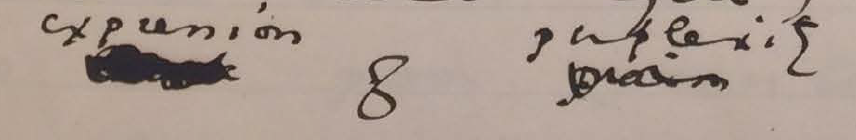
\includegraphics[width=.9\linewidth]{./figure2.png}
\end{center}
Figure 2: Close-up image of detail on MS 9 from The Morgan Library and
Museum. 

\begin{center}
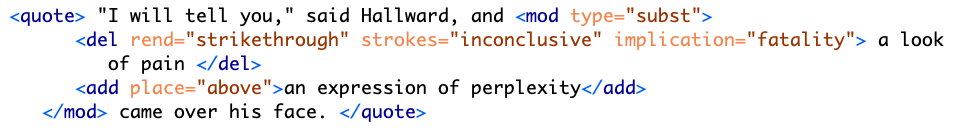
\includegraphics[width=.9\linewidth]{./figure3.png}
\end{center}
Figure 3: Text encoding for page \emph{MS} 9 detail.

My final example concerns a longer passage that was heavily revised in
the manuscript (see Figures 4 and 5). The treatment of this passage
crystallizes the various patterns of revision seen so
far---diminishing signs of intimacy, passion, and references to
Basil's fatalism. The passage in the manuscript bears quoting in
full. Prior to any revisions, it reads:

\#+BEGIN\(_{\text{QUOTE}}\) "You remember that landscape of mine\ldots{} It is one of the
best things I have ever done. And why is it so? Because, while I was
painting it, Dorian Gray sat beside me, and as he leaned across to
look at it, his cheek just brushed my cheek. The world becomes young
to me when I hold his hand, as when I see him, the centuries yield up
all their secrets!"

"Basil, this is [illegible] you must not talk [illegible] [illegible]
his power, [indecipherable] to make yourself the [illegible] slave! It
is worse than wicked, it is silly. I hate Dorian Gray."

Hallward got up from the seat, and walked up and down the garden. A
curious smile curled his lips. He seemed like a man in a dream. After
some time he came back. "You don't understand, Harry\ldots{}" he said.
"Dorian Gray is merely to me a motive in art. He is never more present
in my work then when no image of him is there. He is simply a
suggestion, as I have said, of a new manner. I see him in the curves
of certain lines, in the loveliness and subtleties of certain
colours. That is all."

"Then why won't you exhibit his picture?"

"Because I have put into it the romance of which I have never dared to
speak to him. He knows nothing about it, but the world might guess it,
where there is merely love, they would see something evil, where there
is spectacular passion, they would suggest something vile." (20--21)

\begin{center}
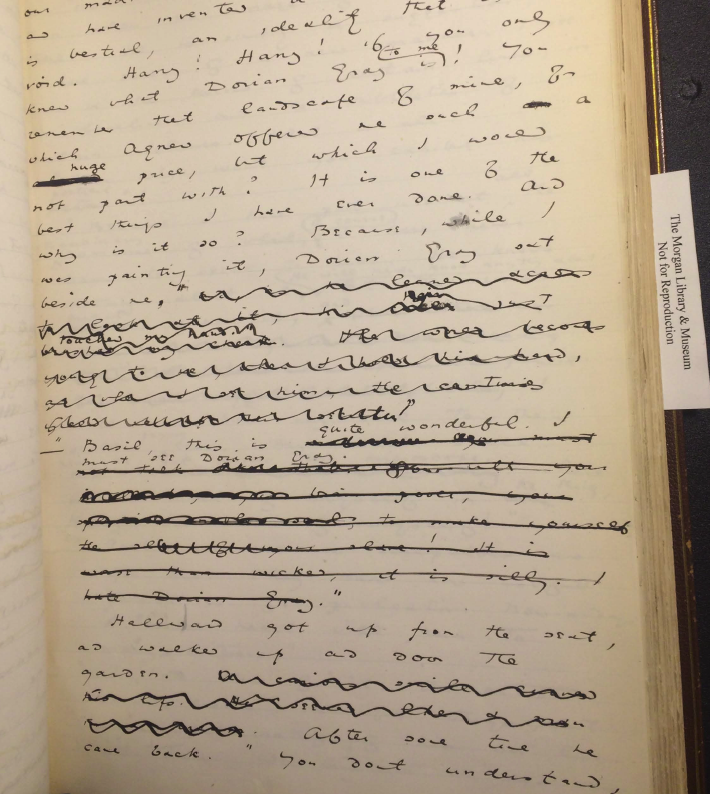
\includegraphics[width=.9\linewidth]{./figure4.png}
\end{center}
Figure 4: \emph{MS} page 20 from The Morgan Library and
Museum. 

\begin{center}
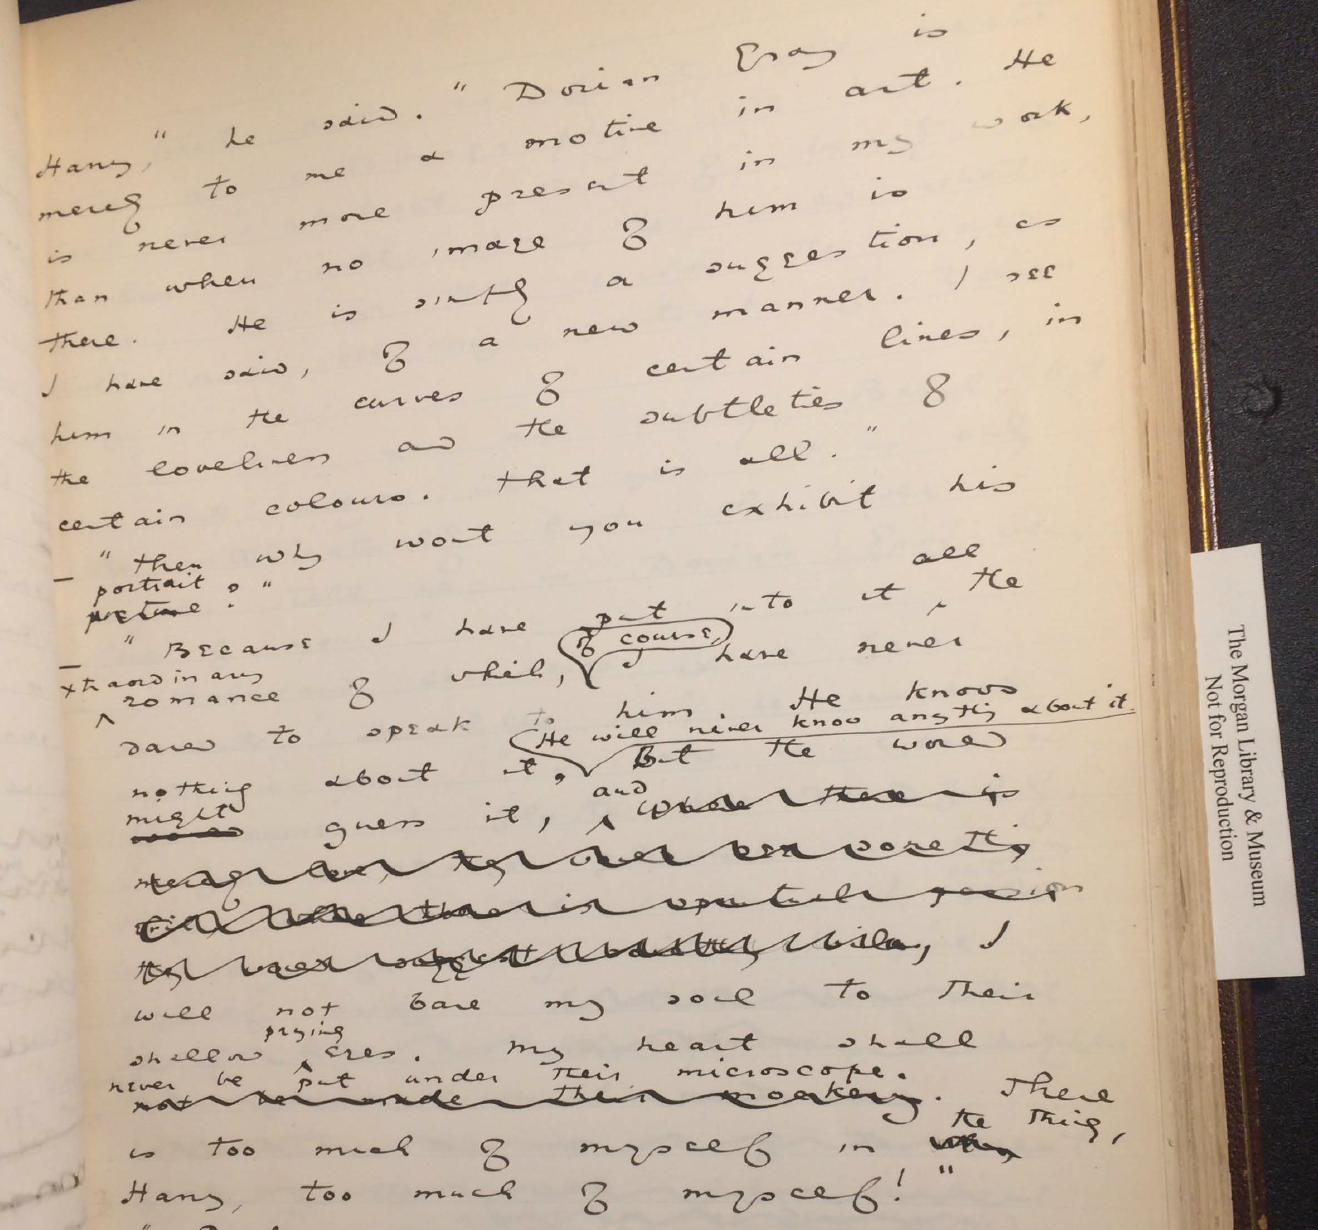
\includegraphics[width=.9\linewidth]{./figure5.png}
\end{center}
Figure 5:/MS/ page 21 from The Morgan Library and
Museum. 

The TEI surfaces Wilde's layers of revision in this passage (see
Figures 6 and 7). In the first paragraph, Wilde eliminates a span of
text from "and as he leaned" to "secrets!". Within this span, Wilde
makes additional changes, adding text such as "hair just touched my
hand". Due to its physical nature, this particular phrase is marked as
"intimacy" in the TEI, while the longer section is enclosed by the
label of "passion," which denotes the nature of the other revisions
within the same sentence, like "The world becomes young to me when I
hold his hand." Here, the TEI enables a layered approach to markup
where one element can be nested within another.

\begin{center}
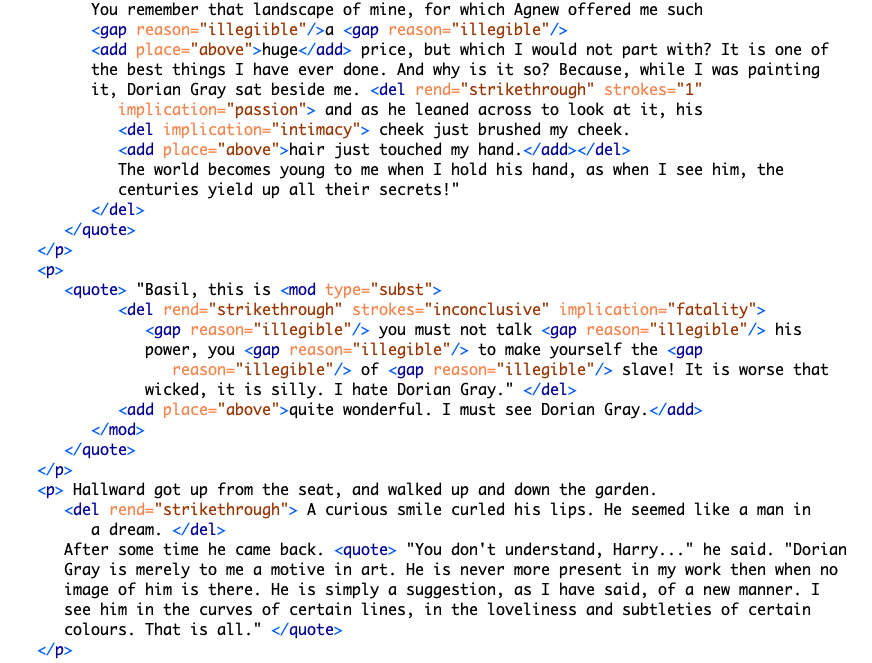
\includegraphics[width=.9\linewidth]{./figure6.png}
\end{center}
Figure 6: Text encoding for \emph{MS} pages 20--21.

\begin{center}
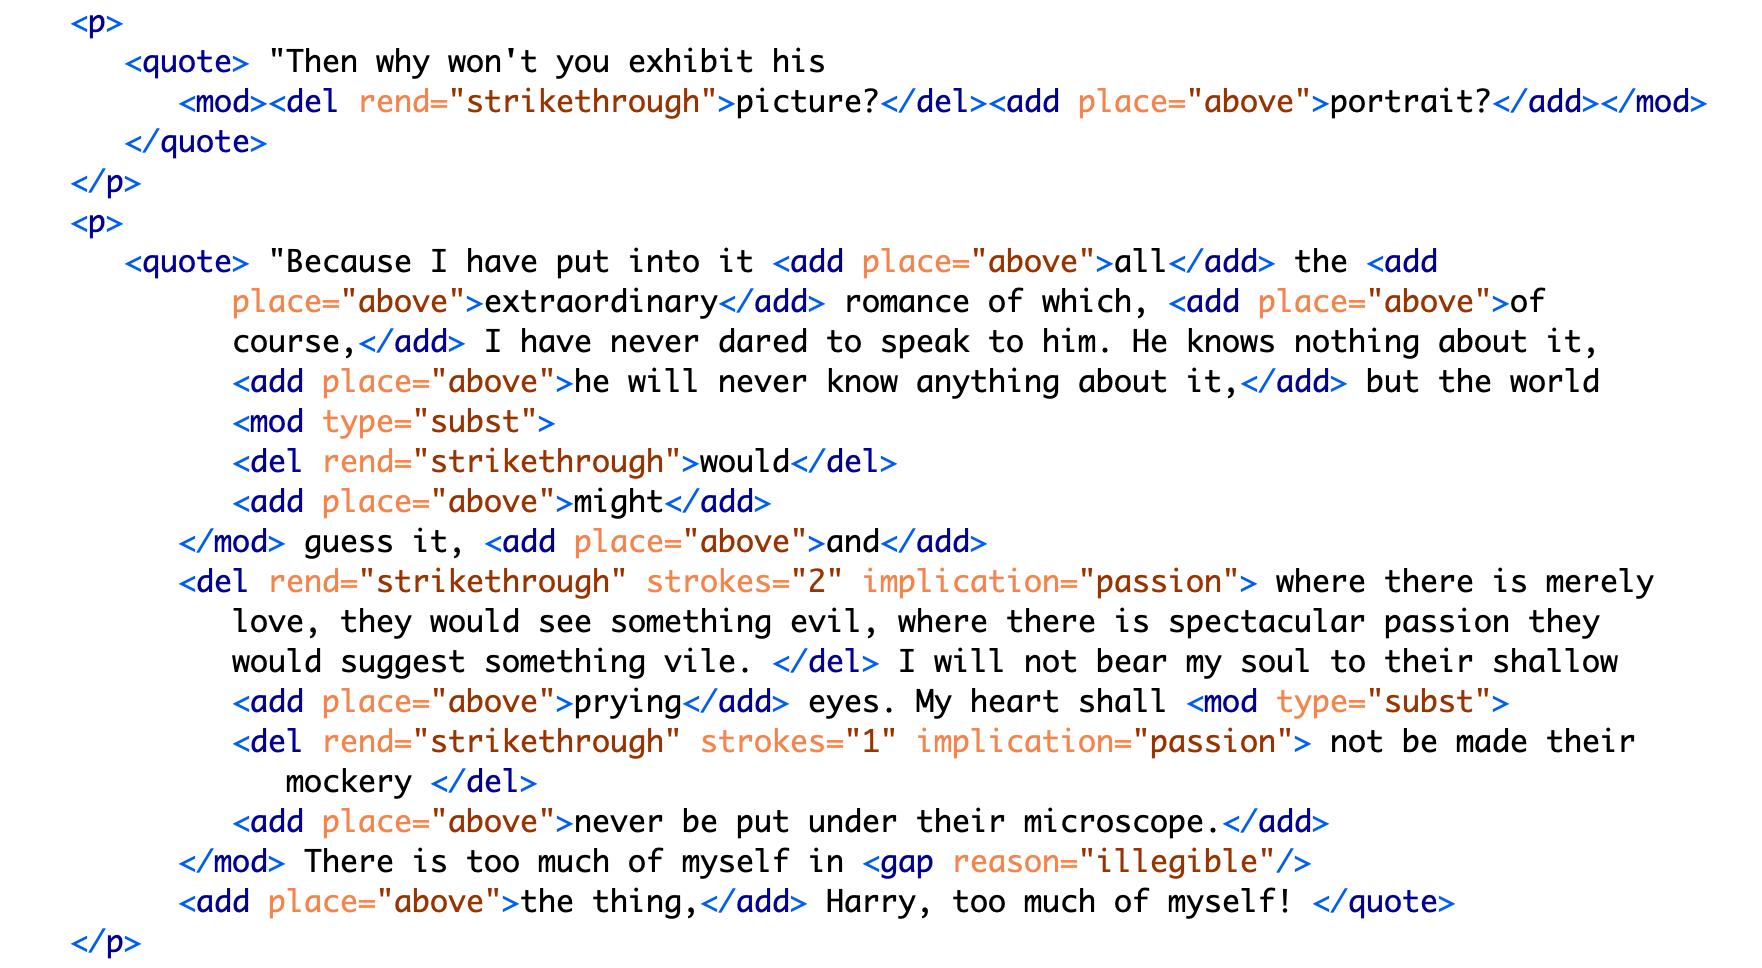
\includegraphics[width=.9\linewidth]{./figure7.png}
\end{center}
Figure 7: Text encoding for \emph{MS} pages 20-21 continued.

While the first paragraph is legible, the next one, by contrast, is
almost completely blotted out. It consists of Lord Henry's
condemnatory and jealous protestations: "his power," "to make yourself
the \ldots{}  slave!" and "I hate Dorian Gray." Here, Wilde obscures the
fatalistic connotations of Basil's passion, which exasperate Lord
Henry.  Accordingly, the \texttt{@implication} is marked as "fatality" and
the \texttt{@strokes} are marked as "inconclusive."

Most of the third paragraph is preserved, presumably for how it
furthers Dorian's aestheticization. Here, Basil elaborates upon
Dorian's aesthetic influence, which inspires his apprehension of the
natural world. In the following paragraph, however, Wilde again
obscures much of language, which revolves around the themes of passion
and fatality. On the theme of fatality, the small adjustment of
"would" to "might" eliminates a sense of inevitability about Basil's
feelings for Dorian.  On the theme of passion, the revelatory line:
"where there is merely love, they would see something evil, where
there is spectacular passion, they would suggest something vile" is
completely struck out. This statement clarifies Dorian's importance
for Basil as the source of a powerful allure that suffuses Basil's art
with beauty. Notably, the strokes over the phrase "suggest something
vile" are doubled, which cannot be encoded in the TEI without
separating the revision into two instances. As with the deletion of
"look of pain" (9), marking each element here with precision would
require separating into distinct entities what is in fact one act of
revision that contains plural implications. It would involve resolving
Wilde's perhaps indeterminate motives into a single intention.

On one level, the TEI encoding reinforces the claim by Lawlor,
Frankel, and Bristow that Wilde diminishes the homoerotic elements by
transforming Dorian from an erotic into an aesthetic object. This goal
is achieved in three ways: first, by easing the tension surrounding
his dialogue with Lord Henry; second, by emphasizing Dorian as an
ideal subject for art; and finally, by removing the destructive
connotations of Basil's attachment to Dorian. On a deeper level,
however, the existing textual scholarship has yet to contend with the
complex ways in which Wilde's intentionality is distributed among the
revisions. To resolve some of the difficulty with encoding this text,
one might employ more precise qualitative markers such as "tension" in
addition to "intimacy," or "ardor" and "devotion," in addition to
"passion," for example. At the same time, however, creating more tags
would dilute the analytical utility of the TEI encoding, which is
meant not meant to be exhaustive. 

In this project, the TEI reveals that the themes of intimacy, beauty,
passion, and fatality operate in intransigent or inscrutable ways:
They may be plural, co-existing within a single line of text; they may
be inextricable, with one enabling the other, like intimacy and
passion which enable fatality; or they might enfold one within the
other, encompassing a plurality of intentions. The TEI, which requires
strict disambiguation, surfaces how these themes work together in ways
that cannot be captured by its data structure.

\subsection{Conclusion}
\label{sec:orgf83e36d}
But this approach toward queer encoding also points to the
ways that larger structures of dominance act as a silent but
structuring force within text. The more that I work with the TEI, the
more I come to realize that the problem with its data model goes
beyond the boundedness of its elements, and toward a dominating,
top-down structure that it imposes on textual "data." At the root of
the TEI's rigidity is its hierarchical document model that propagates
implicit power relations between elements in the document, where each
element within the tree structure subscribes to its parent element and
dominates its subordinate ones. Within this tree-like architecture,
information is not only encapsulated or bound, it is delineated by the
standards of each governing tag, its syntax, model, attributes, and
contents. 

For this text in particular, the dominant force is that of the writer
himself, a writer with nearly every privilege--gender, racial,
financial, cultural, and educational--who imposes a project of
self-censorship into his revision process. But what of other texts
whose writers or subjects do not have the same privileges? Which are
subscribed to larger systems of domination, such historical forces of
dicrimination, exploitation, and oppression? To better understand the
role of dominance in delimiting data forms, it is useful to turn to a
dataset which has been totally dominated by power structures. One such
dataset comprises Jessica Marie Johnson's subject matter in her book
book, \emph{Wicked Flesh: Black Women, Intimacy, and Freedom in the
Atlantic World}. Here Johnson studies the history of black women in
the 17th and 18th century Atlantic world by reading through and
between official documents and historiographical records written by
slave-owning men, traders, and colonial officials. From these recrods,
which "often contain incomplete information," Johnson weaves a history
"in careful and creative ways" (Johnson 5). Her readings of these
documents surface a complicated and nuanced picture of black womens's
lives and how they negotiated their own freedom practices within
white, male, slave-owning male dominated world.

Johnson illustrates two strategies for approaching this dataset: the
first is a strategy of narration, where Johnson interweaves fragments
that, on their own, tell a story of bondage and subjection to
power. She begins by framing each chapter with the story of different
figure from the archive, constructing for the reader a vivid scene
from the woman's life in a way that foregrounds her character and
accomplishment. The first chapter, for example, presents Seignora
Catti, "a wealthy merchant in her own right, [who] had leveraged her
status as the wife of a European against her commercial savvy and the
opportunities and experience of living in the middle ground between
the Atlantic Ocean to the west and the Wolof sovereigns in the east
for her own benefit" (Johnson 16). The notes reveal that the sources
for Catti's biography stem from biographical writings featuring Jean
Barbot, a commercial agent for a French slaving company based in
Senegal. In Johnson's narrative, Barbot's role is delimited to a
supporting character, to a guest at Catti's dinner party whose
presence serves to bring Catti into the foreground.

In addition to narrativizing between the gaps in the record, Johnson
also magnifies and resignifies these gaps. Drawing on Hortense
Spillers work on black female gender ideologies traced to the Middle
Passage, Johnson's project "rejects discourses of black women as
lascivious or wicked, and transmut[e] them into practices of defiance
and pleasure for themselves" (Johnson 10). This work emerges most
provocatively in the way that Johnson handles information that is
absent from the archive, for example, a census that ignores the
presence of black women and girls living in the New Orleans area in
the early 18th century. Reading these absences as "null values,"\footnote{Johnson here draws from Jacob Gaboury's work on resisting
compulsory identification in social media. See Gaboury,
Jacob. "Becoming NULL: Queer Relations in the Excluded Middle." \emph{Women
\& Performance: a Journal of Feminist Theory}. 28:2, 2018. pp. 143-158.}
rather than absent or zero values, Johnson "resist[s] equating the
missing or inapplicable information with black death" (Johnson 2020,
135). Emphasizing thesee "null" values allows Johnson to index where
these women exceed the logics of colonial subjectification:
\begin{quote}
It is possible to see their absence as evidence of either their
perceived nonexistence or lack of importance, or inferior
data-collection practices. It is also possible, however, to hear in
the register's silence the ecstatic shout of black freedom practices
transgressing colonial desires, black people forming maps of kin
between towns and countryside, black women loving each other into free
states that could not be counted by census officials, much less
managed by imperial entities or recorded on manuscript pages. Johnson
143
\end{quote}
By making a space for silence, Johnson can reframe the effects of
absence within the archive. Johnson demonstrates where these women,
who were not counted, "exceed the bounds of colonial power" that is
based on the quantification and commodification of black life. Rather
than reify the dominating narrative of black subjugation or death,
Johnson hints toward the "ways black women sought out profane,
pleasurable, and erotic entanglements as practices of freedom (Johnson
12). The histories of what could have been, which do not fit into
dominant systems of colonial quantification, include the radical
seeking of “joy and pleasure, g[iving] birth, mother[ing] spaces of
care and celebration, and cultivat[ing] expressive and embodied
aesthetic practices to heal from the everyday toil of their laboring
lives” (Johnson 10). These null values allow Johnson to frame
"blackness not as bondage\ldots{} but as future possibility" (Johnson 2020,
10).

Johnson's historiographical project requires more than just assembling
fragments that survive or resignifying the silences in their place; it
requires narrating from what Johnson describes as "a deeper well of
women, communities, practices, strategies, failures, and terrors that
shaped the meaning of freedom and a faith in the possibility of
emancipation" (Johnson 231). Johnson explains,
\begin{quote}
It is from these depths, deeper than exceptional names and silent
registers, that black women remember their mothers, daughters,
godmothers, and aunts. Black communities remember each other, in
family whispers, at altars, and at communion. Historians, bound by
archives, may scrape dusty folios for sources, may question whether
women and girls will appear or worry that when they do appear, they
emerge as legends, myths, and motifs representing more than
themselves. That is not the intellectual tradition this book was
written in. 
\end{quote}
This distinction between record and memory is the key to Johnson's
historiographical method. Memory is a space that, by design, cannot be
recorded or "marked up." Drawing from memory is a way to answer
Hartman's call to "revisit the scene of subjection without replicating
the grammar of violence." Memory, which is maintained by community and
fueled by imagination, is a space that cannot be regulated and
delimited like documents.

How might this historiographical approach for resisting dominance
structures apply to editorial work? Within an extremely delineated set
of records, which contain only minimal data about the lives she
intends to surface, Johnson works to read through and between the gaps
in the record. The TEI might also work with and through gaps, not of a
data structure, but of a larger system of dominance that enables
editorial work in the first place. As electronic editing scholar Amy
Earhart emphasizes, editorial practices are bound by structures deeper
than the TEI data format--institutional support and funding. In order
to pursue a TEI project, researchers need time, money, training, and
access. These obstacles preclude many text encoding projects from
beginning in the first place and limit their ability to succeed. To
highlight the influence of this structure on text encoding work, I
will close by briefly looking at how two projects take what Earhart
describes as a "DIY approach" that defies the structural constraints
of both the institution and the data format (Earhart 2010, 314).

The first project, the \emph{Editing the Eartha M.M. White Collection},
uses community-based strategies to encourage and train beginner
encoders. Based at the University of Florida, this project is contains
an electronic archive of personal correspondence and other documents
related to Eartha M.M. White (1876–1974), the founder of the Clara
White Mission and a leader of Jacksonville, Florida's African American
community. Beginning in a classroom in 2016, this project continues to
grow through the collaborative effort of students, faculty, staff at
UNF, with recent efforts being made to expand into the Jacksonville
community more broadly. To facilitate collaboration on the project,
they share their TEI documents on GitHub, an online space for
publishing digital work (used primarily for collaborating on open
software), and offer detailed, step-by-step instructions for new
editors to get started with text encoding. The introductory guide to
the archive, aimed at all levels of experience, indicates that this
project draws significantly from a non-specialist and community
knowledge.

The second project, \emph{The Peter Still Papers}, strategically deploys a
minimal approach toward text encoding. Based at Rutgers University,
this project collects and publishes correspondence (1850-1875)
relating to former slave Peter Still’s attempts to purchase freedom
for his wife and children in Alabama, and includes letters by William
Lloyd Garrison, Horace Greeley, and Harriet Beecher Stowe. This
"Documentary Edition" makes selective use of tags based on the
TEI-Lite model, with the goal of bringing out a particular narrative
among the papers:
\begin{quote}
Our intention with the markup has been to produce a rough idea of the
\emph{aboutness} of each letter, and not to count every reference to a
person or a place. Consequently, the persName and placeName tags have
been used selectively\ldots{}. in the personography file, we have made an
attempt to include only those people who were significant in Peter
Still’s world, namely family, friends, and people who helped or
hindered him in his mission. \emph{The Peter Still Papers} 2015-2022, "About"
\end{quote}
Their minimalist tagging scheme reflects an inventive approach toward
the structural limitations surrounding the creation of the archive:
first, the scope of the documents themselves, none of which are
written in Still’s hand, reflect what editors describe as "only one
side of a conversation, punctuated by many gaps and omissions" (The
Peter Still Papers 2015-2022, "About). Additionally, like the \emph{Editing
the Eartha M.M. White Collection}, this project draws from a range of
skillsets, specifically from non-specialists in American history, as
"no member of the project team is a historian by training, nor expert
in the period in question" (The Peter Still Papers 2015-2022,
“About”).

Both \emph{Editing the Eartha M.M. White Collection} and the \emph{The Peter
Still Papers} work within limited structures–-institutional and
informational structures–-toward collaborative and community-oriented
encoding approaches. They demonstrate that resistance is not just
another formal experiment, where non-normative bodies challenge
subscription into an oppressive mainstream. It is a political project
that foregrounds that which cannot be incorporated into the
mainstream. 

The answer to Flander's question, "do we need to queer markup, or is
markup already queerable?" seems to be depend on the kind of structure
that the encoder is challenging within the document (2017). For
Wilde's project, the TEI enables an approach toward editing which
surfaces how queerness slips through attempts at demarcation. By
encouraging encoders to impose a level of fixity on the text, the TEI
allows them to discover exactly where queerness eludes
containment. One may examine the formalizations produced by this TEI
schema not for what it reveals about Wilde's intentions, but for how
it releases potential readings of the history of his composition, in
other words, to mark and visualize its queer form: the elusive
affects, repressed desires, and other coded elements of queerness
within this text.

Although this exercise in failed disambiguation is highly productive,
it is circumscribed to the dominance structures working within this
particular text. And self-revision, or even self-censorship, is not
the same as being silenced. The TEI approach to editing tells a
compelling story about Wilde's work in supressing or tranforming the
homoerotic elements in his story. But it does so within a vaccuum of
Wilde's own implicit privilege, particularly his agency in deciding
what to change and how. Wilde's own power here operates as the
dominating force, but one that is easily overlooked or taken for
granted in the name of recovery. The data structure and format may
encourage encoders, as it did this one, to ignore larger systems of
domination operating around the text. If used thoughtfully and
critically, however, the TEI might eventually surface that which
escapes its own structure, in order to suggest, without resolving, the
ever-shifting permutations of power.

\section{References}
\label{sec:org4612143}

Amin, K, Musser, A J and Pérez, R 2017 ‘Queer Form:
Aesthetics, Race, and the Violences of the Social,' ASAP/Journal., (Vol.
2.2, May), 227--239. DOI: 10.1353/asa.2017.0031

Barnett, F, Blas Z, cárdenas, m, Gaboury, J, Johnson, J M and
Rhee, M 2016 ‘QueerOS: A User's Manual,' (eds. Matthew K. Gold and
Lauren Klein). Debates in the Digital Humanities, University of
Minnesota Press. DOI: 10.5749/j.ctt1cn6thb.8

Blas, Z and cárdenas, m 2007--2012. transCoder: A Software
Development Kit.

Bowers, F 1959 Textual \& Literary Criticism. Cambridge:
Cambridge University Press. DOI: 10.1017/CBO9780511552885

Boyd, J A 2014 ‘The Texting Wilde Project: Thoughts on Tools
for a Computer-Assisted Exegisis of a Biographical Corpus,' The Text
Encoding Initiative Conference and Members Meeting 2014. Evanston:
October 22--24.

Caughie, P L, Datskou, E and Parker, R 2018 ‘Storm Clouds on
the Horizon: Feminist Ontologies and the Problem of Gender.' Feminist
Modernist Studies 1.3, 230--242. DOI: 10.1080/24692921.2018.1505819

Flanders, J 2017 ‘Encoding Identity.' Queer Encoding: Encoding
Diverse Identities. The Digital Scholarship Center, Temple University,
April 28.

Flanders, J 1999--2021 ‘What is the TEI?' The Women Writers
Project.

Gaboury, J 2013 ‘A Queer History of Computing.'
\url{Rhizome.org}.

Gaboury, J 2018 ‘Becoming NULL: Queer relations in the
excluded middle.' Women \& Performance: a Journal of Feminist Theory
28.2, 143--158. DOI: 10.1080/0740770X.2018.1473986

Goldberg, J and Menon, M 2005 ‘Queering History.' PMLA, 120.5,
1608--1617. DOI: 10.1632/003081205X73443

Greg, W W 1950--51 ‘The Rationale of Copy-Text.' Studies in
Bibliography, 3, 19--36.

Halperin, D M 2000 ‘How to Do the History of Male
Homosexuality.' GLQ: A Journal of Lesbian and Gay Studies, 6.1, 87--123.
DOI: 10.1215/10642684-6-1-87

Jewell, A 2012 The Willa Cather Archive. University of
Nebraska, Lincoln. 2004--2013.

Lawler, D L 1988 An Inquiry into Oscar Wilde's Revisions of
the Picture of Dorian Gray. New York: Garland Pub.

Leckie, B 2013 ‘The Novel and Censorship in Late-Victorian
England.' The Oxford Handbook of the Victorian Novel, Corby: Oxford
University Press. DOI: 10.1093/oxfordhb/9780199533145.013.0009

Love, H 2009 Feeling Backward: Loss and the Politics of Queer
History. Cambridge: Harvard University Press. DOI: 10.2307/j.ctvjghxr0

McCabe, S 2005 ‘To Be and to Have: The Rise of Queer
Historicism,' GLQ: A Journal of Lesbian and Gay Studies, 11.1, 119--134.
DOI: 10.1215/10642684-11-1-119

>McGann, J 2001 ‘Radiant Textuality: Literary Studies after the
World Wide Web.' Springer. DOI: 10.1007/978-1-137-10738-1

McKenzie, D F 1986 Bibliography and the Sociology of Texts.
Cambridge: Cambridge University Press.

McKerrow, R B 1950 Prolegomena for the Oxford Shakespeare: A
Study in Editorial Method, Oxford: Clarendon Press, 1939.

Ruddick, N 2003 ‘“The Peculiar Quality of my Genius”:
Degeneration, Decadence, and Dorian Gray in 1890--1891.' Robert N Keane
(ed) Oscar Wilde: The Man, His Writings, and His World, New York: AMS
Press, 125--137.

Tanselle, T 1989 A Rationale of Textual Criticism, University
of Pennsylvania Press.

Thain, M 2016 ‘Perspective: Digitizing the Diary --
Experiments in Queer Encoding,' Journal of Victorian Culture, 21.2,
226--241. DOI: 10.1080/13555502.2016.1156014

\emph{The Shelley-Godwin Archive}. University of Maryland, College
Park. Maryland Institute for Technology in the Humanities (MITH).

Traub, V 2013 ‘The New Unhistoricism in Queer Studies.' PMLA,
128.1, 21--39. DOI: 10.1632/pmla.2013.128.1.21

Wilde, O 1889--90 MA 883. The Picture of Dorian Gray:
Original Manuscript. Morgan Library \& Museum, New York, NY.

Wilde, O and Bristow, J 2000 The Complete Works of Oscar
Wilde, 3, Oxford: Oxford University Press. DOI:
10.1093/actrade/9780198119609.book.1

Wilde, O and Frankel, N 2011 The Picture of Dorian Gray: An
Annotated, Uncensored Edition. Cambridge: Harvard University Press. DOI:
10.4159/harvard.9780674068049

Wilde, O and Gillespie, M P 2007 The Picture of Dorian Gray:
Authoritative Texts, Backgrounds, Reviews and Reactions, Criticism, 2nd
ed., New York, W.W. Norton, 2007.
\end{document}
